

\PassOptionsToPackage{unicode=true}{hyperref} % options for packages loaded elsewhere
\PassOptionsToPackage{hyphens}{url}
\PassOptionsToPackage{dvipsnames,svgnames*,x11names*}{xcolor}
%
\documentclass[]{book}
\usepackage{lmodern}
\usepackage{amssymb,amsmath}
\usepackage{ifxetex,ifluatex}
\usepackage{fixltx2e} % provides \textsubscript
\ifnum 0\ifxetex 1\fi\ifluatex 1\fi=0 % if pdftex
  \usepackage[T1]{fontenc}
  \usepackage[utf8]{inputenc}
  \usepackage{textcomp} % provides euro and other symbols
\else % if luatex or xelatex
  \usepackage{unicode-math}
  \defaultfontfeatures{Ligatures=TeX,Scale=MatchLowercase}
\fi
% use upquote if available, for straight quotes in verbatim environments
\IfFileExists{upquote.sty}{\usepackage{upquote}}{}
% use microtype if available
\IfFileExists{microtype.sty}{%
\usepackage[]{microtype}
\UseMicrotypeSet[protrusion]{basicmath} % disable protrusion for tt fonts
}{}
\IfFileExists{parskip.sty}{%
\usepackage{parskip}
}{% else
\setlength{\parindent}{0pt}
\setlength{\parskip}{6pt plus 2pt minus 1pt}
}
\usepackage{xcolor}
\usepackage{hyperref}
\hypersetup{
            pdftitle={The Open Quant Live Book},
            pdfauthor={Thársis T. P. Souza},
            colorlinks=true,
            linkcolor=Maroon,
            filecolor=Maroon,
            citecolor=Blue,
            urlcolor=Blue,
            breaklinks=true}
\urlstyle{same}  % don't use monospace font for urls
\usepackage{geometry}
\geometry{paperwidth=6in, paperheight=9in}
\usepackage{color}
\usepackage{fancyvrb}
\newcommand{\VerbBar}{|}
\newcommand{\VERB}{\Verb[commandchars=\\\{\}]}
\DefineVerbatimEnvironment{Highlighting}{Verbatim}{commandchars=\\\{\}}
% Add ',fontsize=\small' for more characters per line
\usepackage{framed}
\definecolor{shadecolor}{RGB}{248,248,248}
\newenvironment{Shaded}{\begin{snugshade}}{\end{snugshade}}
\newcommand{\KeywordTok}[1]{\textcolor[rgb]{0.13,0.29,0.53}{\textbf{#1}}}
\newcommand{\DataTypeTok}[1]{\textcolor[rgb]{0.13,0.29,0.53}{#1}}
\newcommand{\DecValTok}[1]{\textcolor[rgb]{0.00,0.00,0.81}{#1}}
\newcommand{\BaseNTok}[1]{\textcolor[rgb]{0.00,0.00,0.81}{#1}}
\newcommand{\FloatTok}[1]{\textcolor[rgb]{0.00,0.00,0.81}{#1}}
\newcommand{\ConstantTok}[1]{\textcolor[rgb]{0.00,0.00,0.00}{#1}}
\newcommand{\CharTok}[1]{\textcolor[rgb]{0.31,0.60,0.02}{#1}}
\newcommand{\SpecialCharTok}[1]{\textcolor[rgb]{0.00,0.00,0.00}{#1}}
\newcommand{\StringTok}[1]{\textcolor[rgb]{0.31,0.60,0.02}{#1}}
\newcommand{\VerbatimStringTok}[1]{\textcolor[rgb]{0.31,0.60,0.02}{#1}}
\newcommand{\SpecialStringTok}[1]{\textcolor[rgb]{0.31,0.60,0.02}{#1}}
\newcommand{\ImportTok}[1]{#1}
\newcommand{\CommentTok}[1]{\textcolor[rgb]{0.56,0.35,0.01}{\textit{#1}}}
\newcommand{\DocumentationTok}[1]{\textcolor[rgb]{0.56,0.35,0.01}{\textbf{\textit{#1}}}}
\newcommand{\AnnotationTok}[1]{\textcolor[rgb]{0.56,0.35,0.01}{\textbf{\textit{#1}}}}
\newcommand{\CommentVarTok}[1]{\textcolor[rgb]{0.56,0.35,0.01}{\textbf{\textit{#1}}}}
\newcommand{\OtherTok}[1]{\textcolor[rgb]{0.56,0.35,0.01}{#1}}
\newcommand{\FunctionTok}[1]{\textcolor[rgb]{0.00,0.00,0.00}{#1}}
\newcommand{\VariableTok}[1]{\textcolor[rgb]{0.00,0.00,0.00}{#1}}
\newcommand{\ControlFlowTok}[1]{\textcolor[rgb]{0.13,0.29,0.53}{\textbf{#1}}}
\newcommand{\OperatorTok}[1]{\textcolor[rgb]{0.81,0.36,0.00}{\textbf{#1}}}
\newcommand{\BuiltInTok}[1]{#1}
\newcommand{\ExtensionTok}[1]{#1}
\newcommand{\PreprocessorTok}[1]{\textcolor[rgb]{0.56,0.35,0.01}{\textit{#1}}}
\newcommand{\AttributeTok}[1]{\textcolor[rgb]{0.77,0.63,0.00}{#1}}
\newcommand{\RegionMarkerTok}[1]{#1}
\newcommand{\InformationTok}[1]{\textcolor[rgb]{0.56,0.35,0.01}{\textbf{\textit{#1}}}}
\newcommand{\WarningTok}[1]{\textcolor[rgb]{0.56,0.35,0.01}{\textbf{\textit{#1}}}}
\newcommand{\AlertTok}[1]{\textcolor[rgb]{0.94,0.16,0.16}{#1}}
\newcommand{\ErrorTok}[1]{\textcolor[rgb]{0.64,0.00,0.00}{\textbf{#1}}}
\newcommand{\NormalTok}[1]{#1}
\usepackage{longtable,booktabs}
% Fix footnotes in tables (requires footnote package)
\IfFileExists{footnote.sty}{\usepackage{footnote}\makesavenoteenv{longtable}}{}
\usepackage{graphicx,grffile}
\makeatletter
\def\maxwidth{\ifdim\Gin@nat@width>\linewidth\linewidth\else\Gin@nat@width\fi}
\def\maxheight{\ifdim\Gin@nat@height>\textheight\textheight\else\Gin@nat@height\fi}
\makeatother
% Scale images if necessary, so that they will not overflow the page
% margins by default, and it is still possible to overwrite the defaults
% using explicit options in \includegraphics[width, height, ...]{}
\setkeys{Gin}{width=\maxwidth,height=\maxheight,keepaspectratio}
% Make links footnotes instead of hotlinks:
\DeclareRobustCommand{\href}[2]{#2\footnote{\url{#1}}}
\setlength{\emergencystretch}{3em}  % prevent overfull lines
\providecommand{\tightlist}{%
  \setlength{\itemsep}{0pt}\setlength{\parskip}{0pt}}
\setcounter{secnumdepth}{5}
% Redefines (sub)paragraphs to behave more like sections
\ifx\paragraph\undefined\else
\let\oldparagraph\paragraph
\renewcommand{\paragraph}[1]{\oldparagraph{#1}\mbox{}}
\fi
\ifx\subparagraph\undefined\else
\let\oldsubparagraph\subparagraph
\renewcommand{\subparagraph}[1]{\oldsubparagraph{#1}\mbox{}}
\fi

% set default figure placement to htbp
\makeatletter
\def\fps@figure{htbp}
\makeatother

\usepackage{booktabs}
\usepackage{amsthm}
\usepackage{pdfpages}
\usepackage{graphicx}
\usepackage{mathtools}
\usepackage[]{natbib}
\bibliographystyle{apalike}

\title{The Open Quant Live Book}
\author{Thársis T. P. Souza}
\date{2019-07-06}




\usepackage{amsthm}
\newtheorem{theorem}{Theorem}[chapter]
\newtheorem{lemma}{Lemma}[chapter]
\newtheorem{corollary}{Corollary}[chapter]
\newtheorem{proposition}{Proposition}[chapter]
\newtheorem{conjecture}{Conjecture}[chapter]
\theoremstyle{definition}
\newtheorem{definition}{Definition}[chapter]
\theoremstyle{definition}
\newtheorem{example}{Example}[chapter]
\theoremstyle{definition}
\newtheorem{exercise}{Exercise}[chapter]
\theoremstyle{remark}
\newtheorem*{remark}{Remark}
\newtheorem*{solution}{Solution}
\let\BeginKnitrBlock\begin \let\EndKnitrBlock\end
\begin{document}

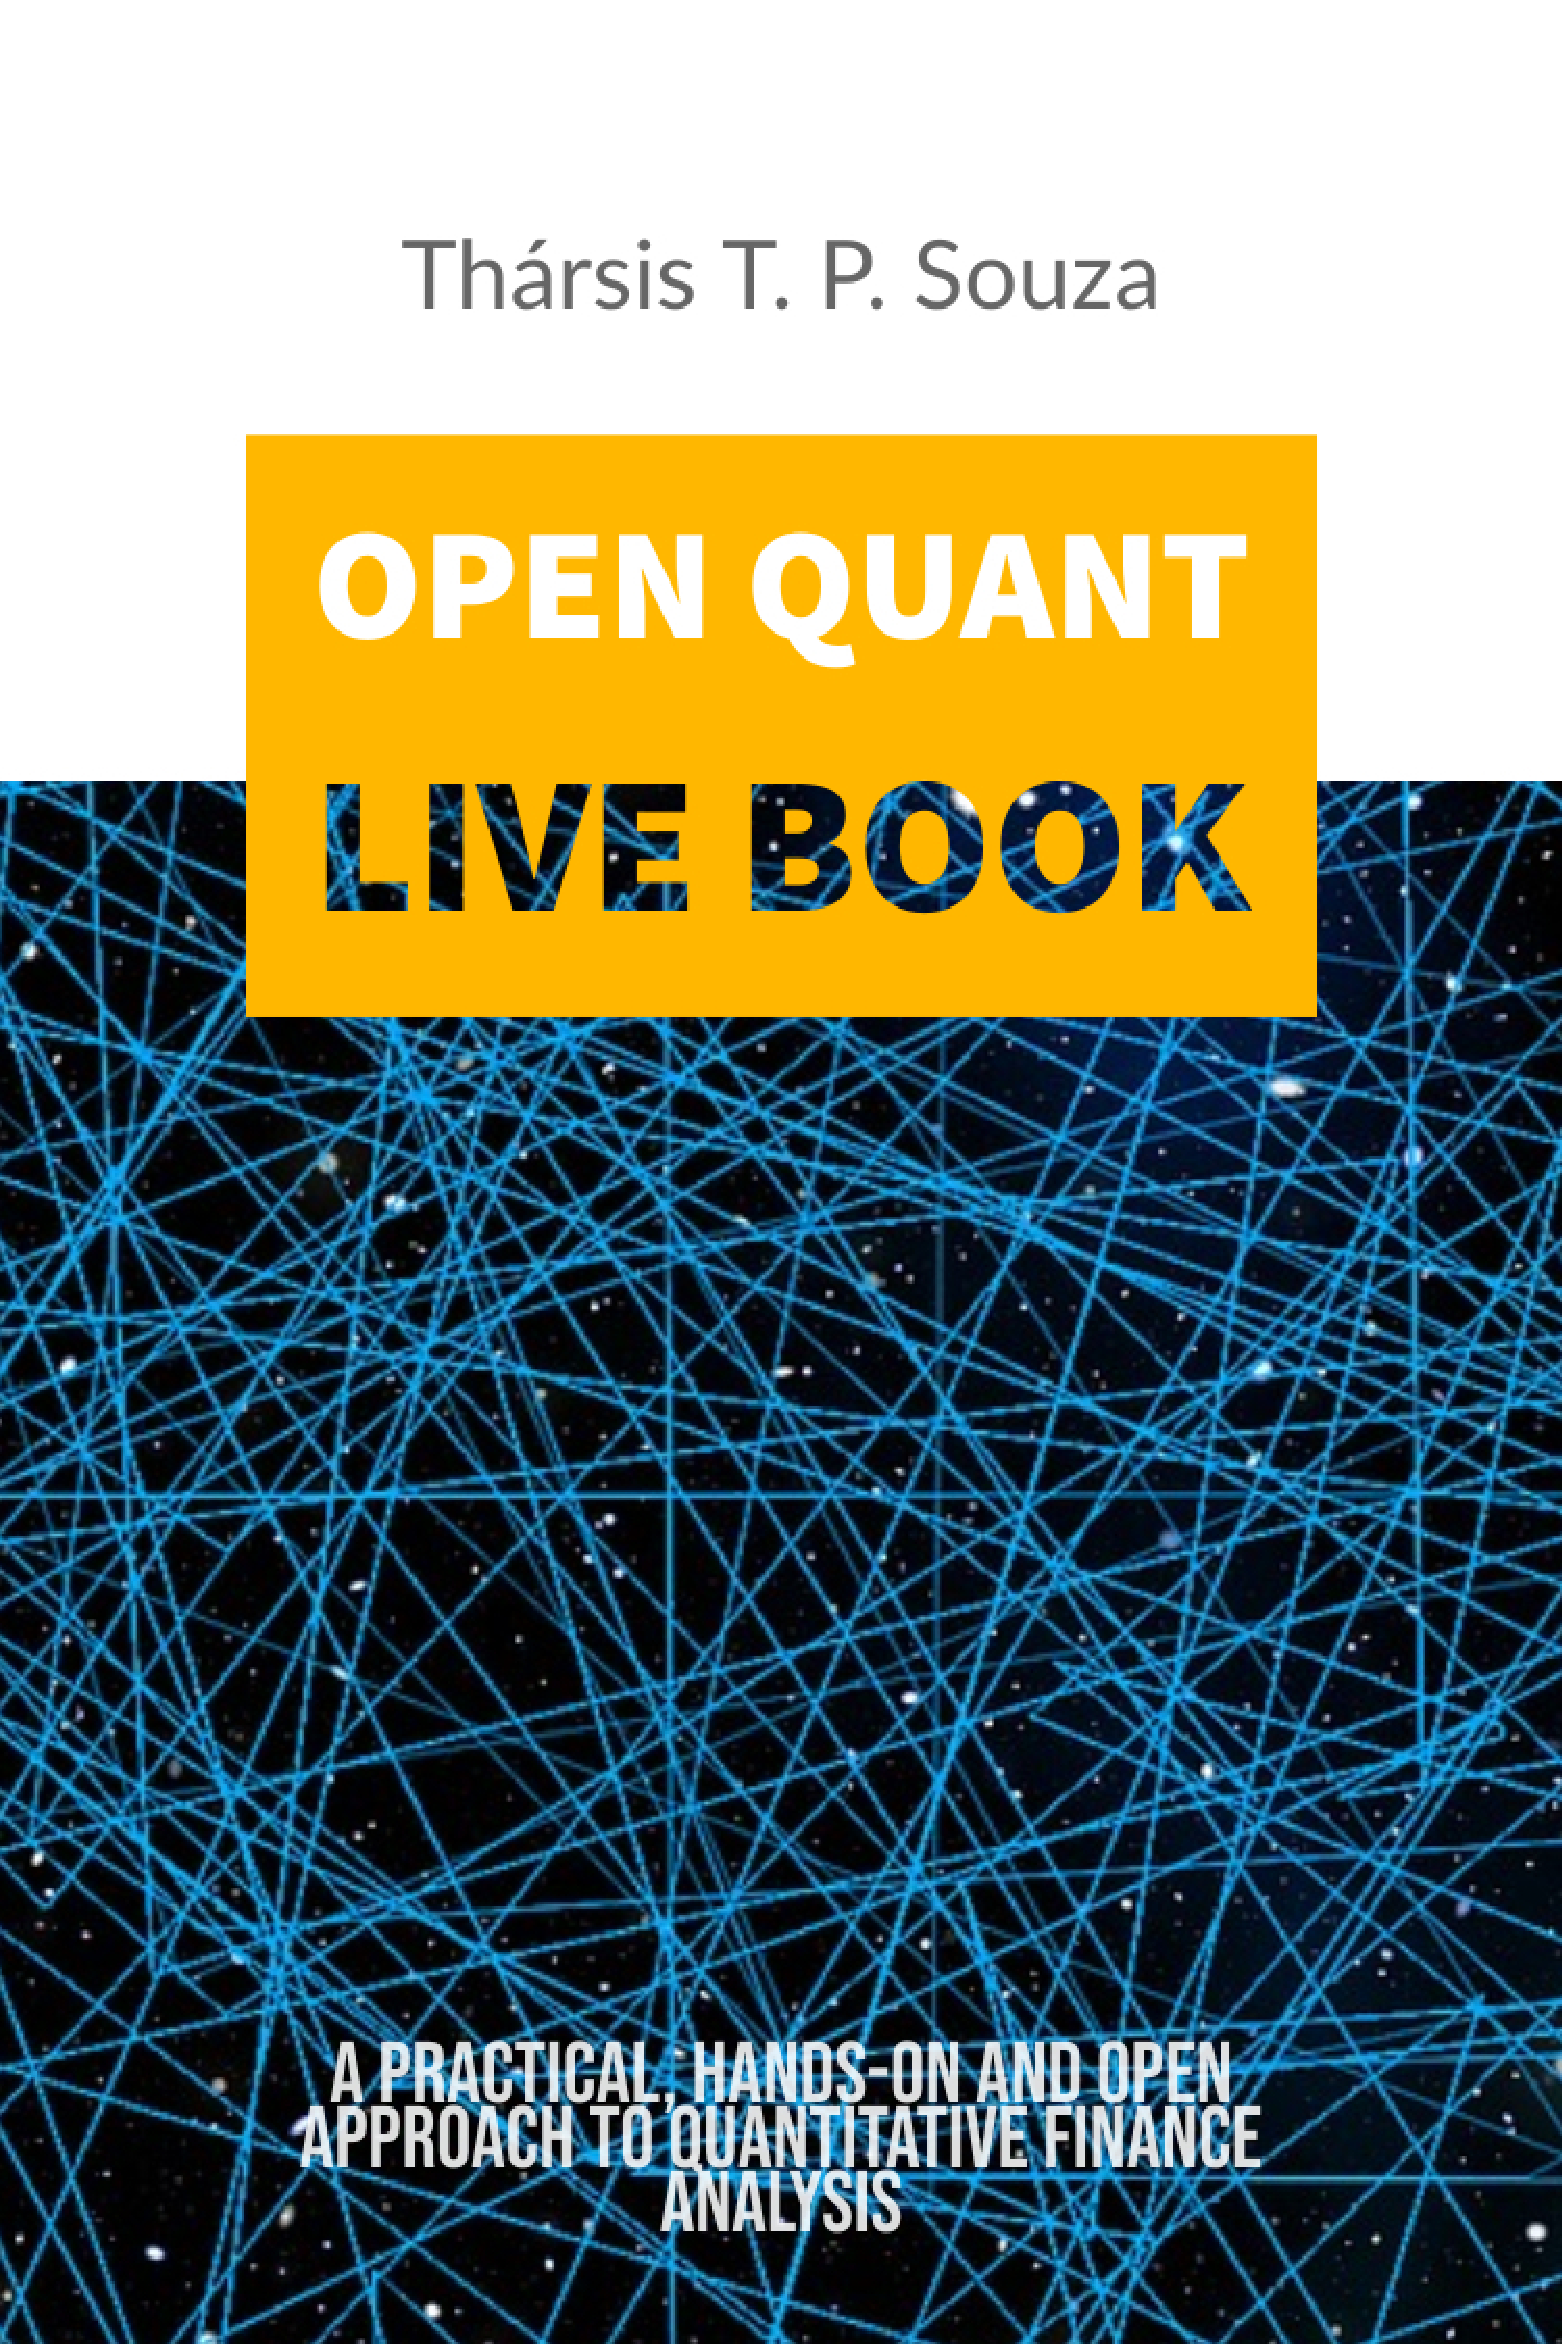
\includepdf{./fig/cover1.pdf}

\maketitle

{
\hypersetup{linkcolor=}
\setcounter{tocdepth}{2}
\tableofcontents
}
\newcommand{\independent}{\perp\!\!\!\!\perp}

\DeclarePairedDelimiter\ceil{\lceil}{\rceil}
\DeclarePairedDelimiter\floor{\lfloor}{\rfloor}

\chapter*{Preface}\label{preface}


\subsection*{Description}\label{description}


The book aims to be an Open Source introductory reference of the most
important aspects of financial data analysis, algo trading, portfolio
selection, econophysics and machine learning in finance with an emphasis
in reproducibility and openness not to be found in most other typical
Wall Street-like references.

The Book is
\href{https://github.com/souzatharsis/open-quant-live-book}{Open} and we
are looking for co-authors. Feel free to
\href{http://www.souzatharsis.com/}{reach out} or simply create a pull
request with your contribution on our
\href{https://github.com/souzatharsis/open-quant-live-book}{Github
project}.

\subsection*{Working Contents}\label{working-contents}


\begin{enumerate}
\def\labelenumi{\arabic{enumi}.}
\tightlist
\item
  The Basics
\end{enumerate}

\begin{itemize}
\tightlist
\item
  I/O
\item
  Stylized Facts
\item
  Correlation \& Causation
\end{itemize}

\begin{enumerate}
\def\labelenumi{\arabic{enumi}.}
\setcounter{enumi}{1}
\tightlist
\item
  Algo Trading
\end{enumerate}

\begin{itemize}
\tightlist
\item
  Investment Process
\item
  Backtesting
\item
  Factor Investing
\item
  Limit Order
\end{itemize}

\begin{enumerate}
\def\labelenumi{\arabic{enumi}.}
\setcounter{enumi}{2}
\tightlist
\item
  Portfolio Optimization
\end{enumerate}

\begin{itemize}
\tightlist
\item
  Modern Portfolio Theory
\item
  Measuring Risk
\item
  Linear Programming
\end{itemize}

\begin{enumerate}
\def\labelenumi{\arabic{enumi}.}
\setcounter{enumi}{3}
\tightlist
\item
  Machine Learning
\end{enumerate}

\begin{itemize}
\tightlist
\item
  Intro
\item
  Agent-Based Models
\item
  Binary Classifiers
\item
  AutoML
\item
  Hierarchical Risk Parity
\end{itemize}

\begin{enumerate}
\def\labelenumi{\arabic{enumi}.}
\setcounter{enumi}{4}
\tightlist
\item
  Econophysics
\end{enumerate}

\begin{itemize}
\tightlist
\item
  Entropy, Efficiency and Coupling
\item
  Transfer Entropy, Information Transfer and Causality
\item
  Financial Networks
\end{itemize}

\begin{enumerate}
\def\labelenumi{\arabic{enumi}.}
\setcounter{enumi}{5}
\tightlist
\item
  Alternative Data
\end{enumerate}

\begin{itemize}
\tightlist
\item
  The Market, The Players, The Rules
\item
  Case Studies
\end{itemize}

\subsection*{Book's information}\label{books-information}


First published at: \href{http://openquants.com/}{openquants.com}.

Licensed under
\href{https://creativecommons.org/licenses/by-nc-sa/4.0/}{Attribution-NonCommercial-ShareAlike
4.0 International}.


\includegraphics[width=0.15\linewidth]{fig/by-nc-sa}

\BeginKnitrBlock{flushright}
Copyright (c) 2019. Thársis T. P. Souza. New York, NY.
\EndKnitrBlock{flushright}

\part{The Basics}\label{part-the-basics}

\chapter{I/O}\label{io}

In this Chapter, we will introduce basic functions to read text, excel
and JSON files as well as large files.

We will also show how to obtain free financial and economic data
including the following:

\begin{itemize}
\tightlist
\item
  End-of-day and real-time pricing;
\item
  Company financials;
\item
  Macroeconomic data.
\end{itemize}

Data sources utilized in this Chapter include the following:

\begin{itemize}
\tightlist
\item
  U.S. Securities and Exchange Commission;
\item
  Quandl;
\item
  IEX;
\item
  Alpha Vantage.
\end{itemize}

\section{Importing Data}\label{importing-data}

\subsection{Text Files}\label{text-files}

The most basic and commonly used option to import data from text files
in R is the use of the function \texttt{read.table} from the
\textbf{r-base}. We can use this function to read text files with
extensions such as \texttt{.txt} and \texttt{.csv}.

\begin{Shaded}
\begin{Highlighting}[]
\NormalTok{dat.table <-}\StringTok{ }\KeywordTok{read.table}\NormalTok{(}\DataTypeTok{file =} \StringTok{"<name of your file>.txt"}\NormalTok{)}
\NormalTok{dat.csv <-}\StringTok{ }\KeywordTok{read.csv}\NormalTok{(}\DataTypeTok{file =} \StringTok{"<name of your file>.csv"}\NormalTok{)}
\end{Highlighting}
\end{Shaded}

The package \textbf{readr} provides functions for reading text data into
R that are much faster that the functions from the \textbf{r-base}. The
\texttt{read\_table} function from the package \textbf{readr} provides a
near-replacement for the \texttt{read.table} function.

\begin{Shaded}
\begin{Highlighting}[]
\KeywordTok{library}\NormalTok{(readr)}
\NormalTok{dat.table <-}\StringTok{ }\NormalTok{readr}\OperatorTok{::}\KeywordTok{read_table2}\NormalTok{(}\DataTypeTok{file =} \StringTok{"<name of your file>.txt"}\NormalTok{)}
\NormalTok{dat.csv <-}\StringTok{ }\NormalTok{readr}\OperatorTok{::}\KeywordTok{read_csv}\NormalTok{(}\DataTypeTok{file =} \StringTok{"<name of your file>.csv"}\NormalTok{)}
\end{Highlighting}
\end{Shaded}

Another option to save data is to write it in \texttt{rds} format. Data
stored in \texttt{rds} format has the advantage to keep the original
data struture and type of the object saved. Also, \texttt{.rds} files
are compressed and consume less space than files saved in \texttt{.csv}
format. A data.frame object can be saved in \texttt{rds} format and then
loaded back as follows:

\begin{Shaded}
\begin{Highlighting}[]
\KeywordTok{write_rds}\NormalTok{(dat.frame, }\DataTypeTok{path =} \StringTok{"<name of your file>.rds"}\NormalTok{)}
\NormalTok{dat.frame <-}\StringTok{ }\KeywordTok{read_rds}\NormalTok{(}\DataTypeTok{path =} \StringTok{"<name of your file>.rds"}\NormalTok{)}
\end{Highlighting}
\end{Shaded}

\subsection{Excel Files}\label{excel-files}

The package \texttt{readxl} has an ease to use interface to functions
that load excel documents in R. The functions \texttt{read\_xls} and
\texttt{read\_xlsx} can be used to read excel files as follows:

\begin{Shaded}
\begin{Highlighting}[]
\KeywordTok{library}\NormalTok{(readxl)}
\NormalTok{readxl}\OperatorTok{::}\KeywordTok{read_xls}\NormalTok{(}\DataTypeTok{path =} \StringTok{"<name of your file>.xls"}\NormalTok{)}
\NormalTok{readxl}\OperatorTok{::}\KeywordTok{read_xlsx}\NormalTok{(}\DataTypeTok{path =} \StringTok{"<name of your file>.xlsx"}\NormalTok{)}
\end{Highlighting}
\end{Shaded}

The function \texttt{read\_excel()} automatically detects the extension
of the input file as follows:

\begin{Shaded}
\begin{Highlighting}[]
\NormalTok{readxl}\OperatorTok{::}\KeywordTok{read_excel}\NormalTok{(}\StringTok{"<name and extension of your file>"}\NormalTok{, }\DataTypeTok{sheet =} \StringTok{"<sheet name or index>"}\NormalTok{)}
\end{Highlighting}
\end{Shaded}

In the \texttt{read\_excel} function, the \texttt{sheet} argument can
receive either the target sheet name or index number, where sheet
indexing starts at 1.

The \texttt{readxl} has been oberving increased use compared to other
comparable packages such as \textbf{gdata} and the \textbf{xlsx} due to
its relative ease of use and performance. Also, the \texttt{readxl} do
not have depency with external code libraries while the packages
\textbf{gdata} and \textbf{xlsx} depend on \texttt{ActiveState\ PERL}
and the \texttt{Java\ JDK}, respectively.

\subsection{JSON Files}\label{json-files}

JSON files are particularly used for transmitting data in web
applications but also frequently used as a standard data interchange
format.

The \texttt{jsonline} package can be used to parse files in JSON format
as follows:

\begin{Shaded}
\begin{Highlighting}[]
\KeywordTok{library}\NormalTok{(jsonlite)}
\NormalTok{result_json <-}\StringTok{ }\KeywordTok{read_json}\NormalTok{(}\StringTok{"<json file>"}\NormalTok{)}
\end{Highlighting}
\end{Shaded}

\subsection{Large Files}\label{large-files}

Fast data manipulation in a short and flexible syntax.

\section{Data Sources}\label{data-sources}

In this section, we will show how to obtain financial and economic data
from public sources.

\subsection{Alpha Vantage}\label{alpha-vantage}

Alpha Vantage offers free access to pricing data including:

\begin{itemize}
\tightlist
\item
  Stock Time Series Data;
\item
  Physical and Digital/Crypto Currencies (e.g., Bitcoin);
\item
  Technical Indicators and
\item
  Sector Performances.
\end{itemize}

The data are available in JSON and CSV formats via REST APIs. The
\textbf{quantmod} and the \textbf{alphavantager} R packages offer a
lightweight R interface to the Alpha Vantage API. Daily stock prices can
be obtained with the \texttt{quantmod::getSymbols} function as follows:

\begin{Shaded}
\begin{Highlighting}[]
\KeywordTok{getSymbols}\NormalTok{(}\DataTypeTok{Symbols =} \StringTok{"AAPL"}\NormalTok{, }\DataTypeTok{src =} \StringTok{"av"}\NormalTok{, }\DataTypeTok{output.size =} \StringTok{"full"}\NormalTok{, }
  \DataTypeTok{adjusted =} \OtherTok{TRUE}\NormalTok{, }\DataTypeTok{api.key =} \StringTok{"your API key"}\NormalTok{)}
\end{Highlighting}
\end{Shaded}

The output data is stored in an object with the same name as the
corresponding symbol, in this example \texttt{AAPL}. The output data
looks like the following

\begin{tabular}{rrrrrr}
\toprule
AAPL.Open & AAPL.High & AAPL.Low & AAPL.Close & AAPL.Volume & AAPL.Adjusted\\
\midrule
13.6 & 16.2 & 13.5 & 16.2 & 6411700 & 0.510\\
16.5 & 16.6 & 15.2 & 15.9 & 5820300 & 0.499\\
15.9 & 20.0 & 14.8 & 18.9 & 16182800 & 0.595\\
18.8 & 19.0 & 17.3 & 17.5 & 9300200 & 0.550\\
17.4 & 18.6 & 16.9 & 18.2 & 6910900 & 0.571\\
\addlinespace
18.1 & 19.4 & 17.5 & 18.2 & 7915600 & 0.571\\
\bottomrule
\end{tabular}

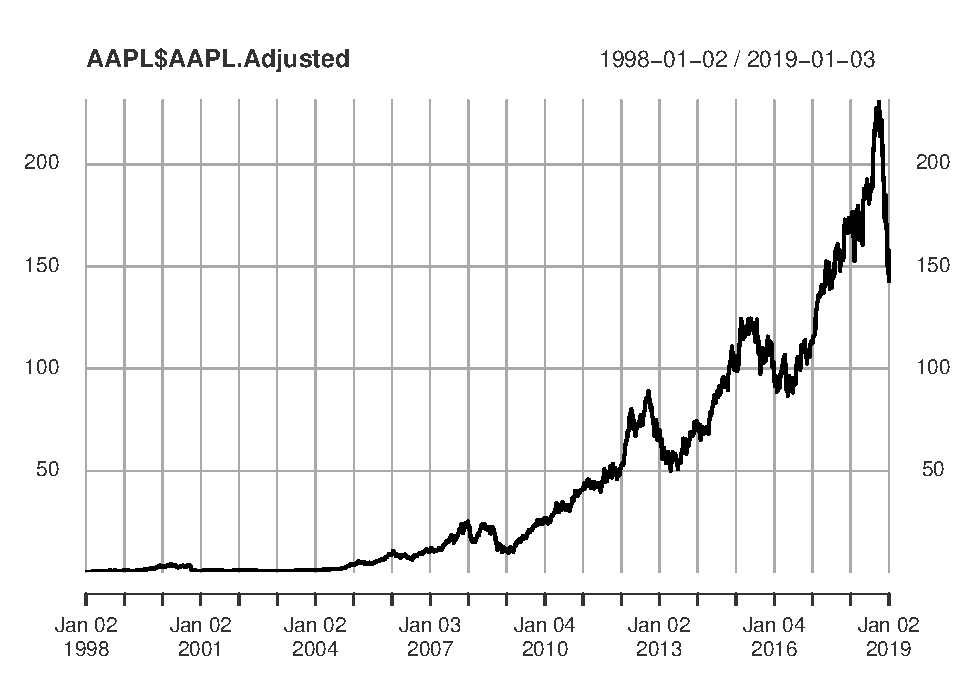
\includegraphics{open-quant-live-book_files/figure-latex/unnamed-chunk-15-1.pdf}

We called the \texttt{quantmod::getSymbols} function with the following
arguments:

\begin{itemize}
\tightlist
\item
  \texttt{Symbols=\textquotesingle{}AAPL\textquotesingle{}} defines a
  character vector specifying the names of each symbol to be loaded,
  here specified by the symbol of the company Apple Inc.;
\item
  \texttt{src="av"} specifies the sourcing method, here defined with the
  value corresponding to Alpha Vantage;
\item
  \texttt{output.size="full"}specified length of the time series
  returned. The strings \texttt{compact} and \texttt{full} are accepted
  with the following specifications: \texttt{compact} returns only the
  latest 100 data points; \texttt{full} returns the full-length time
  series of up to 20 years of historical data;
\item
  \texttt{adjusted=TRUE} defines a boolean variable to include a column
  of closing prices adjusted for dividends and splits;
\item
  \texttt{api.key} specifies your Alpha Vantage API key.
\end{itemize}

\subsection{IEX}\label{iex}

The IEX Group operates the Investors Exchange (IEX), a stock exchange
for U.S. equities that is built for investors and companies. IEX offers
U.S. reference and market data including end-of-day and intraday pricing
data. IEX offers an API with ``a set of services designed for developers
and engineers. It can be used to build high-quality apps and services''.
Data sourced from the IEX API is freely available for commercial subject
to \href{https://iextrading.com/api-exhibit-a/}{conditions} and the use
of their API is subject to additional
\href{https://iextrading.com/api-terms/}{terms of use}.

IEX lists the following github project as an unofficial API for R:
\url{https://github.com/imanuelcostigan/iex}. We will provide examples
on how to obtain intraday pricing data using this package. First, we
will use the \textbf{devtools} to install the package directly from its
github repository as follows:

\begin{Shaded}
\begin{Highlighting}[]
\KeywordTok{library}\NormalTok{(devtools)}
\KeywordTok{install_github}\NormalTok{(}\StringTok{"imanuelcostigan/iex"}\NormalTok{)}
\end{Highlighting}
\end{Shaded}

The \textbf{iex} package provides 4 set of functions as follows:

\begin{itemize}
\tightlist
\item
  \texttt{last}: Provides IEX near real time last sale price, size and
  time. Last is ideal for developers that need a lightweight stock
  quote. \href{https://iextrading.com/developer/docs/\#last}{IEX API
  real time API documentation}.
\item
  \texttt{market}: Provides exchange trade volume data in near real
  time. \href{https://iextrading.com/developer/\#market-market}{IEX
  market API documentation}.
\item
  \texttt{stats}: A set of functions that return trading statistics.
  \href{https://iextrading.com/developer/\#stats}{IEX stats API
  documentation}.
\item
  \texttt{tops}: Provides IEX's aggregated bid and offer position in
  near real time for all securities on IEX's displayed limit order book.
  \href{https://iextrading.com/developer/\#tops-tops}{IEX API TOPS
  documentation}.
\end{itemize}

For instance, the \texttt{last} function has the following arguments:

\begin{itemize}
\tightlist
\item
  \texttt{symbols}: A vector of tickers (case insensitive). Special
  characters will be escaped. A list of eligible symbols is
  \href{https://iextrading.com/trading/eligible-symbols/}{published
  daily} by the IEX. When set to \texttt{NULL} (default) returns values
  for all symbols.
\item
  \texttt{fields}: A vector of fields names to return (case sensitive).
  When set to \texttt{NULL} (default) returns values for all fields.
\item
  \texttt{version}: The API version number, which is used to define the
  API URL.
\end{itemize}

We can obtain intraday stock price data with the \texttt{last} function
as follows:

\begin{Shaded}
\begin{Highlighting}[]
\NormalTok{dat <-}\StringTok{ }\NormalTok{iex}\OperatorTok{::}\KeywordTok{last}\NormalTok{(}\DataTypeTok{symbols =} \KeywordTok{c}\NormalTok{(}\StringTok{"AAPL"}\NormalTok{), }\DataTypeTok{fields =} \KeywordTok{c}\NormalTok{(}\StringTok{"symbol"}\NormalTok{, }
  \StringTok{"price"}\NormalTok{, }\StringTok{"size"}\NormalTok{))}
\end{Highlighting}
\end{Shaded}

The function returns an S3 object of class \texttt{iex\_api} which has
three accessible fields: \texttt{path} , \texttt{response} and
\texttt{content}.

\begin{itemize}
\tightlist
\item
  The \texttt{path} contains the corresponding IEX API path:
\end{itemize}

\begin{Shaded}
\begin{Highlighting}[]
\NormalTok{dat}\OperatorTok{$}\NormalTok{path}
\end{Highlighting}
\end{Shaded}

\begin{verbatim}
## [1] "tops/last"
\end{verbatim}

\begin{itemize}
\tightlist
\item
  The \texttt{response} contains the unparsed IEX API response:
\end{itemize}

\begin{Shaded}
\begin{Highlighting}[]
\NormalTok{dat}\OperatorTok{$}\NormalTok{response}
\end{Highlighting}
\end{Shaded}

\begin{verbatim}
## Response [https://api.iextrading.com/1.0/tops/last?symbols=AAPL&filter=symbol%2Cprice%2Csize]
##   Date: 2019-02-17 23:55
##   Status: 200
##   Content-Type: application/json; charset=utf-8
##   Size: 45 B
\end{verbatim}

\begin{itemize}
\tightlist
\item
  The \texttt{content} contains the parsed content from the API's
  response:
\end{itemize}

\begin{Shaded}
\begin{Highlighting}[]
\NormalTok{dat}\OperatorTok{$}\NormalTok{content}
\end{Highlighting}
\end{Shaded}

\begin{verbatim}
## [[1]]
## [[1]]$symbol
## [1] "AAPL"
## 
## [[1]]$price
## [1] 142
## 
## [[1]]$size
## [1] 100
\end{verbatim}

According to the developer, this package causes R to pause 0.2 seconds
after executing an API call to avoid the user being throttled by the IEX
API (which enforces a 5 request per second limit). Documentation about
the other set of functions can be obtained at
\url{https://github.com/imanuelcostigan/iex/tree/master/man}.

\subsection{Quandl}\label{quandl}

\subsection{SEC}\label{sec}

Official filings are freely available from the U.S. Securities and
Exchange Commission's EDGAR database. The package \texttt{finreportr}
provides an interface in R to facilitate financial analysis from SEC's
10K and 10K/A filings.

We can obtain company basic information with the function the
\texttt{CompanyInfo} function by passing the ticker symbol of the target
company as follows:

\begin{Shaded}
\begin{Highlighting}[]
\KeywordTok{library}\NormalTok{(}\StringTok{"finreportr"}\NormalTok{)}
\NormalTok{AAPL.Info <-}\StringTok{ }\KeywordTok{CompanyInfo}\NormalTok{(}\StringTok{"AAPL"}\NormalTok{)}
\KeywordTok{print}\NormalTok{(AAPL.Info)}
\end{Highlighting}
\end{Shaded}

\begin{verbatim}
##     company        CIK  SIC state state.inc FY.end
## 1 APPLE INC 0000320193 3571    CA        CA   0930
##       street.address         city.state
## 1 ONE APPLE PARK WAY CUPERTINO CA 95014
\end{verbatim}

As a result, we obtain the following information:

\begin{itemize}
\tightlist
\item
  Company name: APPLE INC;
\item
  SEC Central Index Key (CIK): 0000320193;\\
\item
  Standard Industrial Classification (SIC): 3571, which is the industry
  code for Electronic Computers;
\item
  Address: ONE APPLE PARK WAY, CUPERTINO CA 95014;
\item
  Most recent period of report end is 0930.
\end{itemize}

The list of company annual reports with corresponding filing dates can
be obtained with the function \emph{AnnualReports} as follows:

\begin{Shaded}
\begin{Highlighting}[]
\NormalTok{AAPL.reports <-}\StringTok{ }\KeywordTok{AnnualReports}\NormalTok{(}\StringTok{"AAPL"}\NormalTok{)}
\end{Highlighting}
\end{Shaded}

\begin{table}[t]

\caption{\label{tab:unnamed-chunk-23}Sample Annual Reports}
\centering
\begin{tabular}{lll}
\toprule
filing.name & filing.date & accession.no\\
\midrule
10-K & 2018-11-05 & 0000320193-18-000145\\
10-K & 2017-11-03 & 0000320193-17-000070\\
10-K & 2016-10-26 & 0001628280-16-020309\\
10-K & 2015-10-28 & 0001193125-15-356351\\
10-K & 2014-10-27 & 0001193125-14-383437\\
\addlinespace
10-K & 2013-10-30 & 0001193125-13-416534\\
\bottomrule
\end{tabular}
\end{table}

The accession number is a unique identifier that the SEC creates for
each filing.

Company financials are organized into 3 segments: Income Statement,
Balance Sheet and Cash Flow.

\textbf{Income Statement}

Financials from the Income Statement segment can be obtained with the
\emph{GetIncome} function as follows:

\begin{Shaded}
\begin{Highlighting}[]
\NormalTok{AAPL.IS <-}\StringTok{ }\KeywordTok{GetIncome}\NormalTok{(}\StringTok{"AAPL"}\NormalTok{, }\DecValTok{2017}\NormalTok{)}
\end{Highlighting}
\end{Shaded}

\begin{table}[t]

\caption{\label{tab:unnamed-chunk-25}Sample Income Statement Financials}
\centering
\begin{tabular}{lllll}
\toprule
Metric & Units & Amount & startDate & endDate\\
\midrule
Revenue, Net & usd & 233715000000 & 2014-09-28 & 2015-09-26\\
Revenue, Net & usd & 75872000000 & 2015-09-27 & 2015-12-26\\
Revenue, Net & usd & 50557000000 & 2015-12-27 & 2016-03-26\\
Revenue, Net & usd & 42358000000 & 2016-03-27 & 2016-06-25\\
Revenue, Net & usd & 46852000000 & 2016-06-26 & 2016-09-24\\
\addlinespace
Revenue, Net & usd & 215639000000 & 2015-09-27 & 2016-09-24\\
\bottomrule
\end{tabular}
\end{table}

The Income Statement function returns data for the following metrics:

\begin{table}[t]

\caption{\label{tab:unnamed-chunk-26}Income Statement Metrics}
\centering
\begin{tabular}{l}
\toprule
Metrics\\
\midrule
Revenue, Net\\
Cost of Goods and Services Sold\\
Gross Profit\\
Research and Development Expense\\
Selling, General and Administrative Expense\\
\addlinespace
Operating Expenses\\
Operating Income (Loss)\\
Nonoperating Income (Expense)\\
Income (Loss) from Continuing Operations before Income Taxes, Noncontrolling Interest\\
Income Tax Expense (Benefit)\\
\addlinespace
Net Income (Loss) Attributable to Parent\\
Earnings Per Share, Basic\\
Earnings Per Share, Diluted\\
Weighted Average Number of Shares Outstanding, Basic\\
Weighted Average Number of Shares Outstanding, Diluted\\
\addlinespace
Common Stock, Dividends, Per Share, Declared\\
\bottomrule
\end{tabular}
\end{table}

\textbf{Balance Sheet}

Financials from the Balance Sheet segment can be obtained with the
\emph{GetBalanceSheet} function as follows:

\begin{Shaded}
\begin{Highlighting}[]
\NormalTok{AAPL.BS <-}\StringTok{ }\KeywordTok{GetBalanceSheet}\NormalTok{(}\StringTok{"AAPL"}\NormalTok{, }\DecValTok{2017}\NormalTok{)}
\end{Highlighting}
\end{Shaded}

\begin{table}[t]

\caption{\label{tab:unnamed-chunk-28}Sample Balance Sheet Financials}
\centering
\begin{tabular}{lllll}
\toprule
Metric & Units & Amount & startDate & endDate\\
\midrule
Cash and Cash Equivalents, at Carrying Value & usd & 13844000000 & NA & 2014-09-27\\
Cash and Cash Equivalents, at Carrying Value & usd & 21120000000 & NA & 2015-09-26\\
Cash and Cash Equivalents, at Carrying Value & usd & 20484000000 & NA & 2016-09-24\\
Cash and Cash Equivalents, at Carrying Value & usd & 20289000000 & NA & 2017-09-30\\
Available-for-sale Securities, Current & usd & 46671000000 & NA & 2016-09-24\\
\addlinespace
Available-for-sale Securities, Current & usd & 53892000000 & NA & 2017-09-30\\
\bottomrule
\end{tabular}
\end{table}

The Balance Sheet function returns data for the following metrics:

\begin{table}[t]

\caption{\label{tab:unnamed-chunk-29}Balance Sheet Metrics}
\centering
\begin{tabular}{l}
\toprule
Metrics\\
\midrule
Cash and Cash Equivalents, at Carrying Value\\
Available-for-sale Securities, Current\\
Accounts Receivable, Net, Current\\
Inventory, Net\\
Nontrade Receivables, Current\\
\addlinespace
Other Assets, Current\\
Assets, Current\\
Available-for-sale Securities, Noncurrent\\
Property, Plant and Equipment, Net\\
Goodwill\\
\addlinespace
Intangible Assets, Net (Excluding Goodwill)\\
Other Assets, Noncurrent\\
Assets\\
Accounts Payable, Current\\
Accrued Liabilities, Current\\
\addlinespace
Deferred Revenue, Current\\
Commercial Paper\\
Long-term Debt, Current Maturities\\
Liabilities, Current\\
Deferred Revenue, Noncurrent\\
\addlinespace
Long-term Debt, Excluding Current Maturities\\
Other Liabilities, Noncurrent\\
Liabilities\\
Commitments and Contingencies\\
Common Stocks, Including Additional Paid in Capital\\
\addlinespace
Retained Earnings (Accumulated Deficit)\\
Accumulated Other Comprehensive Income (Loss), Net of Tax\\
Stockholders' Equity Attributable to Parent\\
Liabilities and Equity\\
\bottomrule
\end{tabular}
\end{table}

\textbf{Cash Flow}

Financials from the Cash Flow segment can be obtained with the
\emph{GetCashFlow} function as follows:

\begin{Shaded}
\begin{Highlighting}[]
\NormalTok{AAPL.CF <-}\StringTok{ }\KeywordTok{GetCashFlow}\NormalTok{(}\StringTok{"AAPL"}\NormalTok{, }\DecValTok{2017}\NormalTok{)}
\end{Highlighting}
\end{Shaded}

\begin{table}[t]

\caption{\label{tab:unnamed-chunk-31}Sample Cash Flow Financials}
\centering
\begin{tabular}{lllll}
\toprule
Metric & Units & Amount & startDate & endDate\\
\midrule
Cash and Cash Equivalents, at Carrying Value & usd & 13844000000 & NA & 2014-09-27\\
Cash and Cash Equivalents, at Carrying Value & usd & 21120000000 & NA & 2015-09-26\\
Cash and Cash Equivalents, at Carrying Value & usd & 20484000000 & NA & 2016-09-24\\
Cash and Cash Equivalents, at Carrying Value & usd & 20289000000 & NA & 2017-09-30\\
Net Income (Loss) Attributable to Parent & usd & 53394000000 & 2014-09-28 & 2015-09-26\\
\addlinespace
Net Income (Loss) Attributable to Parent & usd & 18361000000 & 2015-09-27 & 2015-12-26\\
\bottomrule
\end{tabular}
\end{table}

The Cash Flow function returns data for the following metrics:

\begin{table}[t]

\caption{\label{tab:unnamed-chunk-32}Cash Flow Metrics}
\centering
\begin{tabular}{l}
\toprule
Metrics\\
\midrule
Cash and Cash Equivalents, at Carrying Value\\
Net Income (Loss) Attributable to Parent\\
Depreciation, Amortization and Accretion, Net\\
Share-based Compensation\\
Deferred Income Tax Expense (Benefit)\\
\addlinespace
Other Noncash Income (Expense)\\
Increase (Decrease) in Accounts Receivable\\
Increase (Decrease) in Inventories\\
Increase (Decrease) in Other Receivables\\
Increase (Decrease) in Other Operating Assets\\
\addlinespace
Increase (Decrease) in Accounts Payable\\
Increase (Decrease) in Deferred Revenue\\
Increase (Decrease) in Other Operating Liabilities\\
Net Cash Provided by (Used in) Operating Activities\\
Payments to Acquire Available-for-sale Securities\\
\addlinespace
Proceeds from Maturities, Prepayments and Calls of Available-for-sale Securities\\
Proceeds from Sale of Available-for-sale Securities\\
Payments to Acquire Businesses, Net of Cash Acquired\\
Payments to Acquire Property, Plant, and Equipment\\
Payments to Acquire Intangible Assets\\
\addlinespace
Payments to Acquire Other Investments\\
Payments for (Proceeds from) Other Investing Activities\\
Net Cash Provided by (Used in) Investing Activities\\
Proceeds from Issuance of Common Stock\\
Excess Tax Benefit from Share-based Compensation, Financing Activities\\
\addlinespace
Payments Related to Tax Withholding for Share-based Compensation\\
Payments of Dividends\\
Payments for Repurchase of Common Stock\\
Proceeds from Issuance of Long-term Debt\\
Repayments of Long-term Debt\\
\addlinespace
Proceeds from (Repayments of) Commercial Paper\\
Net Cash Provided by (Used in) Financing Activities\\
Cash and Cash Equivalents, Period Increase (Decrease)\\
Income Taxes Paid, Net\\
Interest Paid\\
\bottomrule
\end{tabular}
\end{table}

\section{Conclusion}\label{conclusion}

\begin{itemize}
\tightlist
\item
  We showed how to load and import data from both local files and
  external sources.
\item
  We provided examples on how to read tabular data and how to handle
  large files.
\item
  We showed how to obtain financial and economic data from freely
  available sources.
\end{itemize}

\subsection{Further Reading}\label{further-reading}

To further learn how to use R to load, transform, visualize and model
data see \citep{Wickham:2017:RDS:3086927}. Additional relevant R
packages include the following:

\begin{itemize}
\tightlist
\item
  dplyr: Fast data frames manipulation and database query.
\item
  reshape2: Flexibly rearrange, reshape and aggregate data.
\item
  readr: A fast and friendly way to read tabular data into R.
\item
  tidyr: Easily tidy data with spread and gather functions.
\item
  rlist: A toolbox for non-tabular data manipulation with lists.
\item
  jsonlite: A robust and quick way to parse JSON files in R.
\item
  ff: Data structures designed to store large datasets.
\item
  lubridate: A set of functions to work with dates and times.
\end{itemize}

\chapter{Stylized Facts}\label{stylized-facts}

\section{Introduction}\label{introduction}

\section{Distribution of Returns}\label{distribution-of-returns}

\subsection{Fat Tails}\label{fat-tails}

\subsection{Skewness}\label{skewness}

\section{Volatility}\label{volatility}

\subsection{Time-invariance}\label{time-invariance}

\subsection{Volatility Clustering}\label{volatility-clustering}

\subsection{Correlation with Trading
Volume}\label{correlation-with-trading-volume}

\section{Correlation}\label{correlation}

\subsection{Time-invariance}\label{time-invariance-1}

\subsection{Auto-correlation}\label{auto-correlation}

\chapter{Correlation \& Causation}\label{correlation-causation}

\section{Introduction}\label{introduction-1}

\section{A First Definition of
Causality}\label{a-first-definition-of-causality}

We quantify causality by using the notion of the causal relation
introduced by Granger \citep{Wiener56, granger:econ} where a signal
\(X\) is said to Granger-cause \(Y\) if the future realizations of \(Y\)
can be better explained using the past information from \(X\) and \(Y\)
rather than \(Y\) alone.

The most common definitions of Granger-causality rely on the prediction
of a future value of the variable \(Y\) by using the past values of
\(X\) and \(Y\) itself. In that form, \(X\) is said to \emph{G-cause}
\(Y\) if the use of \(X\) improves the prediction of \(Y\).

Let \(X_t\) be a random variable associated at time \(t\) while \(X^t\)
represents the collection of random variables up to time \(t\). We
consider \({X_t}, {Y_t}\) and \({Z_t}\) to be three stochastic
processes. Let \(\hat Y_{t+1}\) be a predictor for the value of the
variable \(Y\) at time \(t+1\).

We compare the expected value of a loss function \(g(e)\) with the error
\(e=\hat{Y}_{t+1} - Y_{t+1}\) of two models:

\begin{enumerate}
\def\labelenumi{\arabic{enumi}.}
\tightlist
\item
  The expected value of the prediction error given only \(Y^t\)

  \begin{equation}
   \mathcal{R}(Y^{t+1} \, | \, Y^t,Z^t) = \mathbb{E}[g(Y_{t+1} - f_1(X^{t},Z^t))]
  \end{equation}
\item
  The expected value of the prediction error given \(Y^t\) and \(X^t\)

  \begin{equation}
   \mathcal{R}(Y^{t+1} \, | \, X^{t},Y^t,Z^t) = \mathbb{E}[g(Y_{t+1} - f_2(X^{t},Y^t,Z^t))].
  \end{equation}
\end{enumerate}

In both models, the functions \(f_1(.)\) and \(f_2(.)\) are chosen to
minimize the expected value of the loss function. In most cases, these
functions are retrieved with linear and, possibly, with nonlinear
regressions. Typical forms for \(g(.)\) are the \(l1\)- or \(l2\)-norms.

We can now provide our first definition of statistical causality under
the Granger causal notion as follows:

\BeginKnitrBlock{definition}
\protect\hypertarget{def:G1}{}{\label{def:G1} }\(X\) does not Granger-cause
\(Y\) relative to side information \(Z\) if and only if
\(\mathcal{R}(Y_{t+1} \; | \; X^t, Y^t, Z^t) = \mathcal{R}(Y_{t+1} \; | \; Y^t, Z^t)\).
\EndKnitrBlock{definition}

A more general definition than Def. \ref{def:G1} that does not depend on
assuming prediction functions can be formulated by considering
conditional probabilities. A probabilistic definition of G-causality
assumes that \(Y_{t+1}\) and \(X^{t}\) are independent given the past
information \((X^{t}, Y^{t})\) if and only if
\(p(Y_{t+1} \, | \, X^{t}, Y^{t}, Z^{t}) = p(Y_{t+1} \, | \, Y^{t}, Z^{t})\),
where \(p(. \, | \, .)\) represents the conditional probability
distribution. In other words, omitting past information from \(X\) does
not change the probability distribution of \(Y\). This leads to our
second definition of statistical causality as follows:

\BeginKnitrBlock{definition}
\protect\hypertarget{def:G2}{}{\label{def:G2} }\(X\) does not Granger-cause
\(Y\) relative to side information \(Z\) if and only if
\(Y_{t+1} \independent X^{t} \; | \; Y^{t}, Z^{t}\).
\EndKnitrBlock{definition}

Def. \ref{def:G2} does not assume any functional form in the coupling
between \(X\) and \(Y\). Nevertheless, it requires a method to assess
their conditional dependency.

In the next Section, we define a parametric linear specification of
G-causality based on Def. \ref{def:G1}. Later in the book, in the
Section \ref{nonlinearG}, when we cover Econophysics techniques, we will
present a nonlinear specification for G-causality based on Def.
\ref{def:G2}.

\section{Quantifying Granger-Causality}\label{LinearG}

We will take the following procedure to quantify Granger-causality
according to Def. \ref{def:G1}:

\begin{enumerate}
\def\labelenumi{\arabic{enumi}.}
\tightlist
\item
  Specify two predictive models:
\end{enumerate}

\begin{itemize}
\tightlist
\item
  The first considers \(Y^t\) to predict \(Y^{t+1}\) (Model
  \(\mathcal{M}\));
\item
  The second considers \(Y^t\) and \(X^t\) to predict \(Y^{t+1}\) (Model
  \(\mathcal{M}^*\));
\end{itemize}

\begin{enumerate}
\def\labelenumi{\arabic{enumi}.}
\setcounter{enumi}{1}
\tightlist
\item
  Test for model misspecification;
\item
  Test the hypothesis that the expected value of the prediction error of
  the Models \(\mathcal{M}\) and \(\mathcal{M}^*\) are statistically the
  same;
\item
  Apply correction for multiple hypothesis testing.
\end{enumerate}

If the null hypothesis from 3. is rejected then there is evidence that
\(X\) Granger-causes \(Y\) under Def. \ref{def:G1}.

\subsection{Model Specification}\label{model-specification}

Standard Granger-causality tests assume a linear relationship among the
causes and effects and are implemented by fitting autoregressive models
\citep{Wiener56, granger:econ}.

Consider the linear vector-autoregressive (VAR) equations:

\begin{align}
Y(t) &= {\alpha} + \sum^k_{\Delta t=1}{{\beta}_{\Delta t} Y(t-\Delta t)} + \epsilon_t, \label{eq:AR11}\\
Y(t) &= \widehat{\alpha} + \sum^k_{\Delta t=1}{{\widehat{\beta}}_{\Delta t} Y(t-\Delta t)} +  \sum^k_{\Delta t=1}{{\widehat{\gamma}}_{\Delta t}X(t-\Delta t)}+ \widehat{\epsilon}_t, \label{eq:AR22}
\end{align}

where \(k\) is the number of lags considered.

From Def \ref{def:G1}, \(X\) does not G-cause \(Y\) if and only if the
prediction errors of \(X\) in the restricted Eq. \eqref{eq:AR11} and
unrestricted regression models Eq. \eqref{eq:AR22} are equal (i.e., they
are statistically indistinguishable).

\subsection{Test for Misspecification}\label{test-for-misspecification}

A statistically significant causality can be reported only if the linear
models from Eqs. \eqref{eq:AR11} and \eqref{eq:AR22} are not misspecified.
For that purpose, we utilize the BDS test \citep{citeulike:9300127} for
the model misspecification.

The BDS test \citep{citeulike:9300127} is used to detect nonlinear
dependence in time series. When applied to the residuals of a linear
model, the BDS tests the null hypothesis that these residuals are
independent and identically distributed. The BDS test is a powerful test
to detect linear misspecification and nonlinearity
\citep{citeulike:9300127, Barnett97asingle-blind}.

Let \(\epsilon_t = (\epsilon_{t=1}, \ldots, \epsilon_{t=n})\) be the
residuals of the linear fitted model and define its \(m\)-embedding as
\(\epsilon_t^m = (\epsilon_{t}, \epsilon_{t-1}, \ldots, \epsilon_{t-m+1})\).
The \(m\)-embedding correlation integral is given by

\begin{align}
C_{m,n}(\Delta \epsilon) = \frac{2}{k(k-1)}\sum_{s = 1}^{t}{\sum_{t=s}^{n}{ \chi(\| \epsilon_s^m - \epsilon_t^m \|, \Delta \epsilon)    }}, \nonumber
\end{align}

and

\begin{align}
C_{m}(\Delta \epsilon) = \lim_{n\to\infty} C_{m,n}(\Delta \epsilon), \nonumber
\end{align}

where \(\chi\) is an indicator function where
\(\chi(\| \epsilon_s^m - \epsilon_t^m \|, \Delta \epsilon) = 1\) if
\(\| \epsilon_s^m - \epsilon_t^m \| < \Delta \epsilon\) and zero,
otherwise.

The null hypothesis of the BDS test assumes that \(\epsilon_t\) is iid.
In this case,

\begin{align}
C_{m}(\Delta \epsilon) = C_{1}(\Delta \epsilon)^m. \nonumber
\end{align}

The BDS statistic is a measure of the extent that this relation holds in
the data. This statistic is given by the following:

\begin{align}
V_{m}(\Delta \epsilon) = \sqrt{n}\frac{C_{m}(\Delta \epsilon) - C_{1}(\Delta \epsilon)^m}{\sigma_m(\Delta \epsilon)}, \nonumber
\end{align}

where \(\sigma_m(\Delta \epsilon)\) can be estimated as described in
\citep{citeulike:9300127}.

The null hypothesis of the BDS test indicates that the model tested is
not misspecified and it is rejected at the 5\% significance level if
\(\|V_m(\Delta \epsilon)\| > 1.96\). The parameter \(\Delta \epsilon\)
is commonly set as a factor of the variance (\(\sigma_\epsilon\)) of
\(\epsilon\).

\subsection{Analysis of Variance}\label{analysis-of-variance}

A one-way ANOVA test is utilized to test if the residuals from Eqs.
\eqref{eq:AR11} and \eqref{eq:AR22} differ from each other significantly.

\subsection{Multiple Hypotheses Testing
Correction}\label{multiple-hypotheses-testing-correction}

When more than one lag \(k\) is tested, a Bonferroni correction is
applied to control for multiple hypotheses testing.

\section{Conclusion}\label{conclusion-1}

\part{Algo Trading}\label{part-algo-trading}

\chapter{Limit Order}\label{limit-order}

\part{Portfolio
Optimization}\label{part-portfolio-optimization}

\part{Machine Learning}\label{part-machine-learning}

\part{Econophysics}\label{part-econophysics}

\chapter{Entropy}\label{entropy}

Let \(X\) be a random variable and \(P_X(x)\) be its probability density
function (pdf). The entropy \(H(X)\) is a measure of the uncertainty of
\(X\) and is defined in the discrete case as follows:

\begin{equation}
H(X) = -\sum_{x \in X}{P_X(x)\log{P_X(x)}}.
\label{eq:H}
\end{equation}

If the \(\log\) is taken to base two, then the unit of \(H\) is the
\textit{bit} (binary digit). We employ the natural logarithm which
implies the unit in \textit{nat} (natural unit of information).

Given a coupled system \((X,Y)\), where \(P_Y(y)\) is the pdf of the
random variable \(Y\) and \(P_{X,Y}\) is the joint pdf between \(X\) and
\(Y\), the joint entropy between \(X\) and \(Y\) is given by the
following:

\begin{equation}
H(X,Y) = -\sum_{x \in X}{\sum_{y \in Y}{P_{X,Y}(x,y)\log{P_{X,Y}(x,y)}}}.
\label{eq:HXY}
\end{equation}

The conditional entropy is defined by the following:

\begin{equation}
H\left(Y\middle\vert X\right) = H(X,Y) - H(X).
\end{equation}

We can interpret \(H\left(Y\middle\vert X\right)\) as the uncertainty of
\(Y\) given a realization of \(X\).

\section{Efficiency and Bubbles in the Crypto and Equity
Markets}\label{efficiency-and-bubbles-in-the-crypto-and-equity-markets}

\section{Quantifying Non-linear Correlation Between Equity and Commodity
Markets}\label{quantifying-non-linear-correlation-between-equity-and-commodity-markets}

\chapter{Transfer Entropy}\label{transfer-entropy}

\section{Introduction}\label{introduction-2}

\section{Nonlinear G-Causality}\label{nonlinearG}

To compute the nonlinear G-Causality, we use the concept of Transfer
Entropy. Since its introduction \citep{PhysRevLett.85.461}, Transfer
Entropy has been recognized as an important tool in the analysis of
causal relationships in nonlinear systems \citep{citeulike:1447442}. It
detects directional and dynamical information
\citep{10.1371/journal.pone.0109462} while not assuming any particular
functional form to describe interactions among systems.

The Transfer Entropy can be defined as the difference between the
conditional entropies:

\begin{equation}
 TE\left(X \rightarrow Y\right \vert Z) =  H\left(Y^F\middle\vert Y^P,Z^P\right) - H\left(Y^F\middle\vert X^P, Y^P,Z^P\right),
\label{eq:TE}
\end{equation}

which can be rewritten as a sum of Shannon entropies:

\begin{align}
TE\left(X \rightarrow Y\right) = H\left(Y^P, X^P\right) - H\left(Y^F, Y^P, X^P\right) + H\left(Y^F, Y^P\right) - H\left(Y^P\right),
\end{align}

where \(Y^F\) is a forward time-shifted version of \(Y\) at lag
\(\Delta t\) relatively to the past time-series \(X^P\), \(Y^P\) and
\(Z^P\). Within this framework we say that \(X\) does not G-cause \(Y\)
relative to side information \(Z\) if and only if
\(H\left(Y^F\middle\vert Y^P,Z^P \right) = H\left(Y^F\middle\vert X^P, Y^P,Z^P\right)\),
i.e., when \(TE\left(X \rightarrow Y,Z^P\right) = 0\).

Empirically, we reject this null hypothesis of causality if the Transfer
Entropy from \(X\) to \(Y\) is significantly higher than the shuffled
version of the original data.

For this we estimate 400 replicates of
\(TE(X_{Shuffled} \rightarrow Y)\), where \(X_{Shuffled}\) is a random
permutation of \(X\) relatively to \(Y\). We compute the randomized
Transfer Entropy at each permutation for each time-shift (\(\Delta t\))
from 1 to 10 days. We then calculated the frequency at which the
observed Transfer Entropy was equal or more extreme than the randomized
Transfer Entropy. The statistical significance was assessed using
p-value \(< 0.05\) after Bonferroni correction.

\section{The Link Between Linear Granger-causality and Transfer
Entropy}\label{the-link-between-linear-granger-causality-and-transfer-entropy}

It has been shown \citep{PhysRevLett.103.238701} that linear G-causality
and Transfer Entropy are equivalent if all processes are jointly
Gaussian. In particular, by assuming the standard measure (\(l2\)-norm
loss function) of linear G-causality for the bivariate case as follows
(see Section \ref{LinearG} for more details on linear-Granger
causality):

\begin{equation}
GC_{X \rightarrow Y} = \log\left( \frac{var(\epsilon_t)}{var( \widehat{\epsilon}_t)} \right),
\label{eq:GCGC}
\end{equation}

the following can be proved \citep{PhysRevLett.103.238701}:

\begin{align}
TE_{X \rightarrow Y} = GC_{X \rightarrow Y}/2.
\label{eq:GCGC2}
\end{align}

This result provides a direct mapping between the Transfer Entropy and
the linear G-causality implemented in the standard VAR framework. Hence,
it is possible to estimate the TE both in its general form and with its
equivalent form for linear G-causality.

\section{Net Information Flow}\label{net-information-flow}

Transfer-entropy is an asymmetric measure, i.e.,
\(T_{X \rightarrow Y} \neq T_{Y \rightarrow X}\), and it thus allows the
quantification of the directional coupling between systems. The Net
Information Flow is defined as

\begin{equation}
\widehat{TE}_{X \rightarrow Y} = TE_{X \rightarrow Y} - TE_{Y \rightarrow X}\;.
\end{equation}

One can interpret this quantity as a measure of the dominant direction
of the information flow. In other words, a positive result indicates a
dominant information flow from \(X\) to \(Y\) compared to the other
direction or, similarly, it indicates which system provides more
predictive information about the other system
\citep{Michalowicz:2013:HDE:2601840}.

In the next sections we will provide empirical examples that show that
Transfer Entropy can capture information flow in both linear and
nonlinear systems.

\section{Empirical Experiment: Information Flow on Simulated
Systems}\label{empirical-experiment-information-flow-on-simulated-systems}

In this section, we construct simulated systems and test the nonlinear
and linear formulations of the net information flow. We show that only
the nonlinear formulation of net information flow is able to capture the
nonlinear relationships in the simulated systems.

For the nonlinear case, we compute Transfer Entropy as defined in Eq.
\eqref{eq:TE}. Conversely, to estimate the linear version of the Net
Information Flow, we computed the Transfer Entropy using Eq.
\eqref{eq:GCGC2}, i.e., by estimating linear G-causality Eq. \eqref{eq:GCGC}
under a linear-VAR framework.

\section{Empirical Experiment: Information Flow on Global
Markets}\label{empirical-experiment-information-flow-on-global-markets}

\chapter{Financial Networks}\label{financial-networks}

\section{Introduction}\label{introduction-3}

Financial markets can be regarded as a complex network in which nodes
represent different financial assets and edges represent one or many
types of relationships among those assets. Filtered correlation-based
networks have successfully been used in the literature to study
financial markets structure particularly from observational data derived
from empirical financial time series
\citep[\citet{Tumminello26072005}]{bardoscia2017pathways, 10.1371/journal.pone.0017994, Mantegna1999, aste2010correlation, Tumminello201040}.
The underlying principle is to use correlations from empirical financial
time series to construct a sparse network representing the most relevant
connections. Analyses on filtered correlation-based networks for
information extraction \citep{song2008analysis, aste2010correlation}
have widely been used to explain market interconnectedness from
high-dimensional data. Applications include asset allocation
\citep{LI2018, pozzi2013spread}, market stability assessments
\citep{morales2012dynamical}, hierarchical structure analyses
\citep{Mantegna1999, aste2010correlation, Tumminello201040, musmeci2014clustering, song2012hierarchical}
and the identification of lead-lag relationships
\citep{curme2015coupled}.

In this Chapter we will describe how to

\begin{itemize}
\tightlist
\item
  Construct and filter financial networks;
\item
  Build price-based dynamic industry taxonomies;
\item
  Implement a trading strategy based on financial network structure.
\end{itemize}

\section{Network Construction}\label{network-construction}

We selected \(N = 100\) of the most capitalized companies that were part
of the S\&P500 index from 09/05/2012 to 08/25/2017. The list of these
companies' ticker symbols is reported in the Appendix \ref{sec:comps}.
For each stock \(i\) the financial variable was defined as the daily
stock's log-return \(R_i(\tau)\) at time \(\tau\).

Stock returns \(R_i\) and social media opinion scores \(O_i\) each
amounted to a time series of length equals to 1251 trading days. These
series were divided time-wise into \(M = 225\) windows
\(t = 1, 2, \ldots, M\) of width \(T = 126\) trading days. A window step
length parameter of \(\delta T = 5\) trading days defined the
displacement of the window, i.e., the number of trading days between two
consecutive windows. The choice of window width \(T\) and window step
\(\delta T\) is arbitrary, and it is a trade-off between having analysis
that is either too dynamic or too smooth. The smaller the window width
and the larger the window steps, the more dynamic the data are.

To characterize the synchronous time evolution of assets, we used equal
time Kendall's rank coefficients between assets \(i\) and \(j\), defined
as

\begin{equation}
 \rho_{i, j}(t) = \sum\limits_{t' < \tau}sgn(V_i(t') - V_i(\tau))sgn(V_j(t') - V_j(\tau)),
\end{equation}

where \(t'\) and \(\tau\) are time indexes within the window \(t\) and
\(V_i \in \{R_i, O_i\}\).

Kendall's rank coefficients takes into account possible nonlinear
(monotonic) relationships. It fulfill the condition
\(-1 \leq \rho_{i, j} \leq 1\) and form the \(N \times N\) correlation
matrix \(C(t)\) that served as the basis for the networks constructed in
this work. To construct the asset-based financial and social networks,
we defined a distance between a pair of stocks. This distance was
associated with the edge connecting the stocks, and it reflected the
level at which they were correlated. We used a simple non-linear
transformation \(d_{i, j}(t) = \sqrt{2(1 - \rho_{i,j}(t))}\) to obtain
distances with the property \(2 \geq d_{i,j} \geq 0\), forming a
\(N \times N\) symmetric distance matrix \(D(t)\).

\subsection{Network Filtering: Asset
Graphs}\label{network-filtering-asset-graphs}

We extract the \(N(N-1)/2\) distinct distance elements from the upper
triangular part of the distance matrix \(D(t)\), which were then sorted
in an ascending order to form an ordered sequence
\(d_1(t), d_2(t), \ldots, d_{N(N-1)/2}(t)\). Since we require the graph
to be representative of the market, it is natural to build the network
by including only the strongest connections. This is a network filtering
procedure that has been successfully applied in the construction of
\textit{asset graphs} for the analyses of market structure
\cite{1402-4896-2003-T106-011, refId0-Onnela-2004}. The number of edges
to include is arbitrary, and we included those from the bottom quartile,
which represented the 25\% shortest edges in the graph (largest
correlations), thus giving
\(E(t) = \{d_1(t), d_2(t), \ldots, d_{\floor{N/4}}(t)\}\).

We denoted \(E^{F}(t)\) as the set of edges constructed from the
distance matrix derived from stock returns \(R(t)\). The financial
network considered is \(G^{F} = ( V, E^{F} )\), where \(V\) is the
vertex set of stocks.

\subsection{Network Filtering: MST}\label{network-filtering-mst}

\subsection{Network Filtering: PMFG}\label{network-filtering-pmfg}

\section{Applications}\label{applications}

\subsection{Industry Taxonomy}\label{industry-taxonomy}

\subsection{Portfolio Construction}\label{portfolio-construction}

\part{Alternative Data}\label{part-alternative-data}

\chapter{The Market, The Players and The
Rules}\label{the-market-the-players-and-the-rules}

\section{The Market}\label{the-market}

\section{The Data}\label{the-data}

\section{The Buyers}\label{the-buyers}

\section{Conclusion}\label{conclusion-2}

\appendix \addcontentsline{toc}{chapter}{\appendixname}


\chapter{Statistical Methods}\label{statistical-methods}

This Appendix provides details to some of statistical methods used in
the book.

\section{Kernel Density Estimation}\label{kde}

In the entropy computation (see Section \ref{entropy}) the empirical
probability distribution must be estimated. Histogram-based methods and
kernel density estimations are the two main methods for that.
Histogram-based is the simplest and most used nonparametric density
estimator. Nonetheless, it yields density estimates that have
discontinuities and vary significantly depending on the bin size choice.

Also known as the Parzen-Rosenblatt window method, the kernel density
estimation (KDE) approach approximates the density function at point
\(x\) using neighboring observations. However, instead of building up
the estimate according to the bin edges as in histograms, the KDE method
uses each point of estimation \(x\) as the center of a bin of width
\(2h\) and weight it according to a kernel function. Thereby, the kernel
estimate of the probability density function \(f(x)\) is defined as

\begin{equation}
\hat{f} = \frac{1}{nh}\sum_{x' \in X}{K\left(\frac{x - x'}{h}\right)}. 
\label{eq:pdf}
\end{equation}

A usual choice for the kernel \(K\), which we use here, is the
(Gaussian) radial basis function:

\begin{equation}
K(x) = \frac{1}{\sqrt{2\pi}}\exp^{-\frac{1}{2}x^2}. 
\end{equation}

The problem of selecting the bandwidth \(h\) in Eq. \eqref{eq:pdf} is
crucial in the density estimation. A large \(h\) will oversmooth the
estimated density and mask the structure of the data. On the other hand,
a small bandwidth will reduce the bias of the density estimate at the
expense of a larger variance in the estimates. If we assume that the
true distribution is Gaussian and we use a Gaussian kernel, the optimal
value of \(h\) that minimizes the mean integrated squared error (MISE)
is

\begin{equation*}
h^* = 1.06\sigma N^{-1/5},
\end{equation*}

where \(N\) is the total number of points and \(\sigma\) can be
estimated as the sample standard deviation. This bandwidth estimation is
often called the Gaussian approximation or Silverman's rule of thumb for
kernel density estimation \citep{silverman}. This is the most
commonly-used method and it is here employed. Other common methods are
given by \citep{sheather1991reliable} and \citep{scott1992multivariate}.

\bibliography{book.bib,packages.bib}

\end{document}
